\section{Architecture}

\subsection{Stakeholders}

\subsubsection{Customer}
Our goal with this course was to create a product that not only works the way the customer intended, but with satisfactory performance. Our code needed to be written following the clean coding standard and make use of interfaces and general polymorphism, so that their developers could further develop this solution with ease.

\subsubsection{Course Evaluator}
For us to achieve a good grade, the course evaluator needs to be satisfied. This means that we need to have satisfied the other stakeholders and delivered a well written report with good documentation of our process.

\subsubsection{Supervisor}
In our first meeting with our supervisor, we were told that he would fight for our grade given that he was satisfied. This entails completing the project and delivering a well written report, as well as good under-way documentation.

\subsubsection{Implementers}
The architecture should be easy to implement and make sense to the coders, both those of our own team in addition to those of the customer.

\subsection{Quality Attributes}
The customer was very specific when it came to what they wanted.
\subsubsection{Modifiability}
The solution we were to create making will be used for other ads than real estate ads, therefore we need to make it modifiable so other developers later on can further develop using our solution as a base.
\subsubsection{Performance}
We wanted the system to perform with a satisfactory performance. The customer did not set any specific requirements for performance. For this reason, we decided to merely strive to achieve this goal by writing as efficient code as we could, and otherwise not worry much about it. %Is this too casual?
\subsubsection{Availability}
The system should be available for the users when they need it.
\subsubsection{Interoperability}
Needs to inter-operate with already-existing order system. This goal will be achieved by using the technology the customer tells us to use, including Web API and MSSQL and so on.
\subsubsection{Readability}
The customer wants us to write readable code. We are supposed to do a polymorphy/interface type of programming so it's easier for other developers to extend via plugins etc. therefore it's important that the code is readable so other's can easily understand what's going on without much hazzle.

\subsection{Views}


\subsubsection{Process view}
There is no need for us to supply a process view, because we do not have access to their server. We are only supposed to write the code for their system, without taking into account how the processes interoperate.
\subsubsection{Logical view}
\begin{figure}[h]
\centering
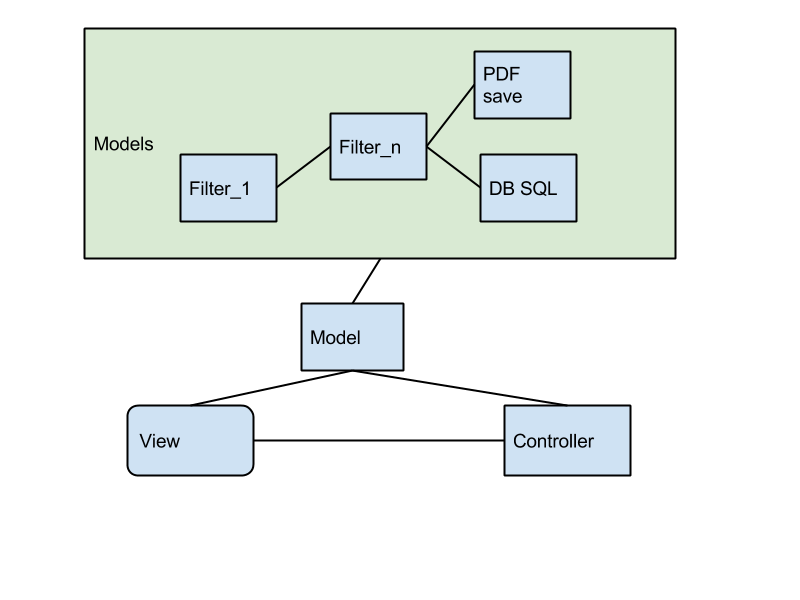
\includegraphics[width=0.8\textwidth]{images/architecture00.png}
\caption{Logical view}
\label{fig:logical_view}
\end{figure}
\newpage

\subsubsection{Scenario view}
\begin{figure}[h]
\centering
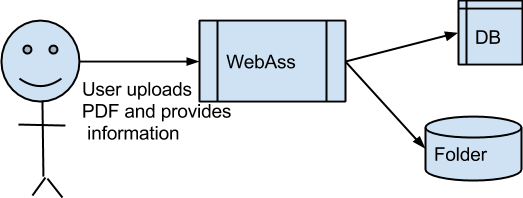
\includegraphics[width=0.8\textwidth]{images/architecture01.png}
\caption{Scenario view}
\label{fig:scenario_view}
\end{figure}


\subsubsection{Physical view}
\begin{figure}[h]
\centering
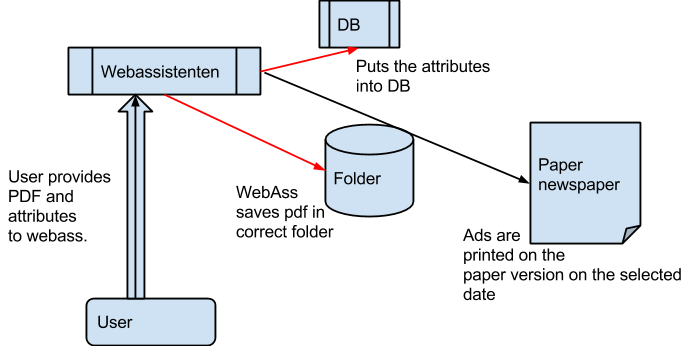
\includegraphics[width=0.8\textwidth]{images/architecture02.png}
\caption{Physical view, we implement the red arrows}
\label{fig:physical_view}
\end{figure}
\newpage
\subsection{Class diagram}
From these views, we made this class diagram.
\begin{figure}[h]
\centering
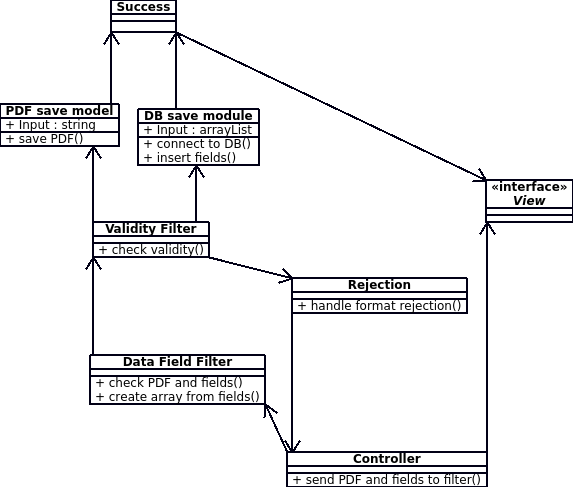
\includegraphics[width=0.8\textwidth]{diagrams/class_diagram.png}
\caption{Digital class diagram}
\label{fig:class_diagram}
\end{figure}
\subsection{Patterns}
MVC due to the technology and pipe \&  filter to filter the data and due to the modifiability requirement.
\subsection{Tactics}
\subsubsection{Modifiability}
\begin{itemize}
\item Increase semantic cohesion
\item Decrease coupling
\item Split modules
\end{itemize}

\subsubsection{Performance}
\begin{itemize}
\item Write optimal code
\end{itemize}

\subsubsection{Availability}
\begin{itemize}
\item Our code should not crash the customer's system, but it's their responsibility that the system is available.
\end{itemize}

\subsubsection{Interoperability}
\begin{itemize}
\item The technology and tools we're using should be sufficient to ensure interoperability
\end{itemize}

\subsubsection{Readability}
\begin{itemize}
\item We will follow the clean coding principle and use camelCase coding. Refer to the Templates and Standards section.
\end{itemize}